\section{Introduction}

Wikiparse is a tree-based approach to representing Wikipedia pages using tightly connected nodes to allow for flexible connections between both visible and invisible information available on a page (such as a link and the page it points to). Data is cached as raw wikitext and as JSON, both for speed and for flexibility, allowing other libraries to use the produced JSON instead of the front-end Python module, if desired. The tree-based layout of pages and the caching of parsed data results in Wikiparse being both much faster and much more capable than similar libraries. This opens the door for using Wikipedia in new ways more easily to further research into Natural Language Processing (NLP).

% Write last

\section{Background and Related Work}

% RESEARCH AGAIN, see old emails

\subsection{Wikipedia for Natural Language Processing}

Wikipedia is a valuable corpus for NLP research. Many of its documents are highly structured and thoroughly reviewed by humans, and it provides a breadth of information with a level of structural consistency not easily found elsewhere, at no cost to researchers. For the purpose of extracting information from Wikipedia pages, it is important that a page's contents are both easy to parse and that as little information as possible gets lost. If information exists in the Wikipedia page, then an NLP application may wish to access that information, and ought to be able to do so easily.

\subsection{Available Solutions}

For the purposes of this paper, the following list will be limited to a few API's easily available to Python. However, non-Python solutions were considered as well and faced similar problems. A more complete list can be found on MediaWiki's list of alternative parsers\cite{altparsers}.

\subsubsection*{MediaWiki API}

The online-interface through MediaWiki's public API\cite{mediawikiapi} is the official standard for parsing wikitext. However, its output is fully formatted HTML, including templates (such as images or sidebars) in the same page as the main page content. The result is a page that is difficult to parse consistently and poorly suited for use in NLP applications. There are alternative ways of using the API, allowing for retrieval of pages as plaintext or getting summary information, such as lists of links or references, but no way to get the wikitext of a page parsed into anything more informative than plaintext.

\subsubsection*{Wikipedia Python Module}

The standard Python Wikipedia module\cite{pywikimodule} offers support for plaintext Wikipedia pages broken by section, with a small set of other features, such as listing links in a page or only retrieving part of the introduction to a page. It delimits sections the same way wikitext does---by using headers bracketed in equals signs---allowing for the text to be reliably divided, but requiring some minor post-processing. However, it completely separates the text from the information associated with that text. For example, while all internal links are made available as a list, there is no way to identify what text was associated with each link. In fact, the information made available through this module is nearly identical to that made available through the MediaWiki API, though it is certainly easier to use in Python applications.

\subsubsection*{JWPL}

JWPL\cite{jwpl} is a powerful Java toolset for downloading and managing Wikipedia archive files, with some support for parsing wikitext into Java objects. Since Java-to-python adaptation libraries exist and are relatively straightforward (the \emph{py4j} and \emph{jpype} Python libraries can both accomplish this), then JWPL can be considered easily Python-usable. Its abilities to optimize archives into database files and manage multiple revisions across time are quite impressive, but its lack of recent support (the latest work on it seems to be from 2012) and its minimalist documentation make it difficult to use even in Java and prone to falling out of date, if it hasn't already. Most significant is its deprecation of parsing wikitext, which makes it an unreliable solution for parsing and comprehending wikitext.

\subsection{Limitations of Solutions}

Converting Wikipedia pages into plaintext is simple, but an enormous amount of information is lost by doing so. Getting access to the content of a Wikipedia page as easy-to-use plaintext, yet without losing non-textual information (such as links or references) is a surprisingly difficult task, and without a custom caching framework, many Wikipedia libraries rely solely on fetching data live from Wikipedia, which can be unacceptably slow for large numbers of pages. In addition, many Wikipedia API's will only provide certain sets of data, such as lists of links and images, but provide no easy way to associate this with text (which may be desired for Named Entity Recognition, for example), and provide no way to obtain unexpected information from the page (perhaps the user is interested in bold and italicized text instead of links).

Most solutions parse wikitext into an HTML output. This is considered an invalid solution to the problem in this paper, since the HTML would then have to be re-parsed to extract information, which could have been done directly from Wikipedia in the first place. For this reason, such solutions are not considered in this paper. These, then, are the three most common problems with the remaining solutions:

\begin{enumerate}
\item They disassociate text-bound information from the text itself (e.g., a link's target from its display text, or a section header from its body).
\item They include no built-in caching, nor a simplified method of pre-caching data.
\item Any text-extracted information provided is inflexible to the actual desires of the library user, potentially throwing away desired information.
\end{enumerate}

\section{Wikiparse Overview}

% Describe usage pattern

Wikiparse is a Python 3 toolset for pre-caching and accessing Wikipedia pages, using a Java post-processor for the Sweble\cite{sweble} parser to convert wikitext into an easily parsable JSON format. It uses a tree structure for pages that preserves context and meaning for every element of a wikitext page, and uses indexed text properties to uniquely identify formatting and text groups, such as lists or bold regions. Both the wikitext and the post-processed JSON are stored in compressed files in a directory tree on the user's filesystem to offer a fast and powerful way to store the millions of pages from a Wikipedia archive file without running extra background systems, such as a database management system, and without using excessive disk space. Also included are simple tools for finding and handling Wikipedia archives to allow even novices with the Wikipedia archive system to find and begin using an archive, although live-fetching of pages is also supported for use without downloading the entirety of Wikipedia.

To obtain or learn to use the toolset, see Appendix \ref{wpcodeanddocs}.

\subsection{Parsing with Sweble}

The most significant part of Wikiparse is the ability to parse and present the content of wikitext as a coherent code object. To do this, Wikiparse uses a thin Java post-processing shell around the Sweble\cite{sweble} wikitext parsing library (also built in Java) that converts the resulting Abstract Syntax Tree (AST) into a simpler tree that can be exported as JSON for common usage. The JSON result is passed directly back to the main Wikiparse library through a py4j client-server setup. Wikiparse only launches this conversion server when it is needed, and only launches it once per run, saving time when converting multiple pages to JSON.

The simpler tree relies on two concepts: contexts and properties. Contexts are nodes that contain a list of other nodes, though most context types have attributes of their own; for example, internal links to other Wikipedia pages are represented as a context with a target attribute, where the content of the context is the list of textual elements that constitute the hyperlink text. Most of the leaves of the context trees are textual elements marked with a list of properties, such as ``bold'' or ``list''. These properties are assigned unique identifiers, allowing multiple text objects to be grouped that share the same bold block, since a single bold directive in wikitext may affect multiple text elements.

By separating context types from textual properties, it is easy to distinguish elements whose type prescribes metadata or structured information (for example, the target of a link, or the name-value pair in a template argument) from those elements whose type is self-descriptive and requires no further information (bold, or list item).

Every object output by the parser is assigned a unique identification number (separate from those used to identify property groups). This allows for an object to be represented just once in JSON, but for it to appear in multiple locations. Doing this enables, for example, the easy grouping of all internal links or external references as ``pointer'' objects in the JSON, dictionaries whose only attribute is the ID number of the element that's being referred to. Like pointers in object-oriented computer languages, this allows a single object (or node in the JSON tree) to be defined once and referred to in as many places as needed.

\subsection{Guided Pre-caching}

Included in the Wikiparse toolset are two directly runnable scripts for pre-caching from Wikipedia archives for the Wikiparse library. Note that pre-caching is not at all necessary for using Wikiparse, but when using a large number of pages, it can provide a significant speed increase.

\subsubsection*{Wikidownloader}

The wikidownloader script is a small helper script that transparently navigates the Wikipedia archive system online, simplifying the decisions to be made and offering help to understand what options are available and what they mean. See Appendix \ref{wdsample} for an example of how this script works. After using this script, the user will have the link or links needed to download the desired Wikipedia archive, which they can unzip manually or let the wikisplitter script unzip for them.

\subsubsection*{Wikisplitter}

The wikisplitter script is a streaming unpacker that can extract the wikitext of pages from a Wikipedia archive without loading the entire archive into memory at once. The script includes the gzip decompression module if needed, but is also capable of running on the decompressed XML file directly, should the user want or need to decompress the archive themselves. The extracted wikitext pages are saved as compressed text files into a tree of directories, based on the page titles. The directory tree ensures that any single directory only immediately contains a few hundred or thousand files at most, and a file's path is immediately known based on its title without any searching.

% wikidownloader
% wikisplitter

\subsection{Cache On Demand}

For users who prefer not to pre-cache the entirety of Wikipedia using these two scripts, Wikiparse can fetch wikitext live from Wikipedia as pages are requested. The textual content used by Wikiparse, including both the wikitext and the parsed JSON version of the wikitext, is automatically cached in compressed files in the user-configurable cache directory. The JSON files are always created on demand by launching (on the first time only) the Java application built around Sweble and passing the wikitext through it. This requires that users have Java installed and in their path, but enables the user to obtain the JSON version of a page without any manual work. Since both the wikitext and JSON for a page can be built and cached transparently, users gain both the ease of not needing anything downloaded to start using Wikiparse, and the speed boost of having pages load quickly when used multiple times.

% filemanager

\subsection{Simplified Content Usage}

Wikipedia pages can be loaded directly from their title, and are represented in Python using a WikiPage object tree. The tree structure allows for selection of what text is desired by the role it plays and its hierarchical position in the page as a whole. This allows for a tree-traversal technique for moving around a WikiPage, without losing the simplicity of thinking of the page as plaintext, since any node can be converted to plaintext on demand.

\begin{figure}[!t]
\centering
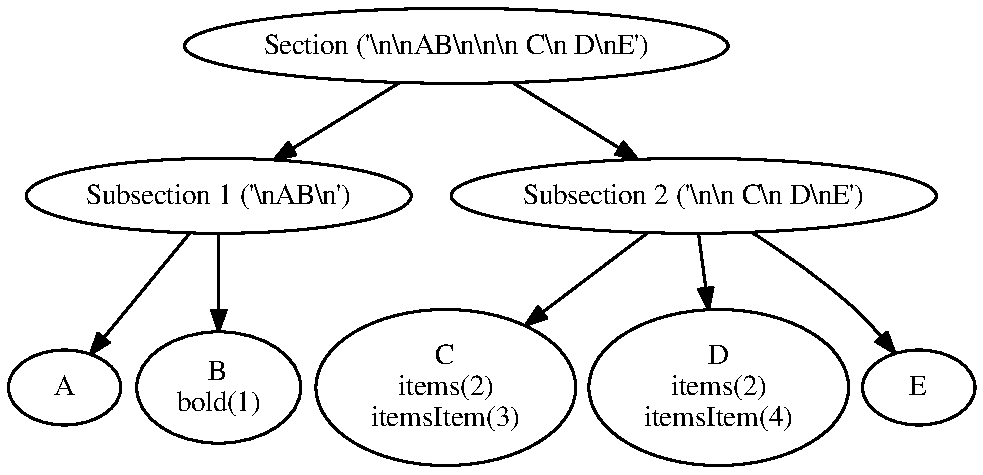
\includegraphics[width=3.5in]{wikiparse_demo_graph}
\caption{Sample Parsed Tree}
\label{sampletree}
\end{figure}

As an example, consider the following fake Wikipedia page:
\begin{verbatim}
= Section =
== Subsection 1 ==
A'''B'''
== Subsection 2 ==
* C
* D
E
\end{verbatim}
This example page generates the tree represented in figure \ref{sampletree}, with newlines excluded for brevity. Nodes are distinct Python objects, where children are included in their parents as an array of content. Section headers, and similar non-body but related information, is included as an attribute of the context to which it belongs. The hierarchy of sections is clearly evident, as is the identification and labelling of textual properties. Obviously far more types exist than those demonstrated here, both for contexts and text properties, but this graph gives the general layout of how the WikiPage is represented as a tree.

Pages on Wikipedia often exhibit more than just a simple textual body. On many pages, sidebars and panels often provide highly detailed and specific information, such as a landmark's geographical location or an organization's website. These are bundled in wikitext as templates with name-value pairs as arguments to the template. Such panels are potentially valuable but also problematic, since they are visible but don't belon in any particular location in the text of the page. To handle this issue without loss of information, a WikiPage object will store each template into its own object in a list of all templates, and each argument contained in the template can be queried using its name and value properties.

Any node, including a single text node, can be converted to a string, or to a custom RichText object. Since the string is simply derived from the RichText object and can be obtained with Python's standard \verb|str| function on either a node in the WikiPage tree or that's node's RichText object, it will be no further discussed, and this paper will assume from here that any node can be easily converted to a string. The generation of a RichText object from a node performs a pre-order depth-first search in that node, resulting in a flat list of tuples containing output text (that would be visible on the Wikipedia page) paired with the node object from which it came, as represented in figure \ref{strblock}. This RichText object is indexed identically to its string, where each index returns the same character as would be obtained from that index of its string form, paired (in a tuple) with the node object that contributed the string from which that character came, as shown in figure \ref{strindiv}.

\begin{figure}[!t]
\centering
\begin{subfigure}{.225\textwidth}
  \centering
  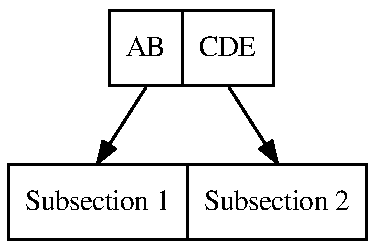
\includegraphics[width=1.5in]{string_graph2}
  \caption{Internal layout of RichText}
  \label{strblock}
\end{subfigure}%
\begin{subfigure}{.225\textwidth}
  \centering
  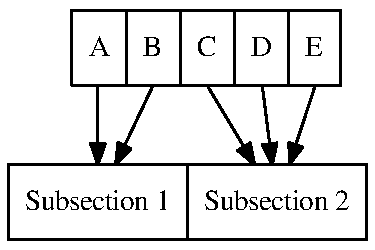
\includegraphics[width=1.5in]{string_graph}
  \caption{Indexing of RichText}
  \label{strindiv}
\end{subfigure}
\caption{RichText object layouts}
\end{figure}

% digraph tree {
% Section [label="Section ('\\n\\nAB\\n\\n\\n C\\n D\\nF')"]
% Subsection1 [label="Subsection 1 ('\\nAB\\n')"]
% Subsection2 [label="Subsection 2 ('\\n\\n C\\n D\\nF')"]
% Section -> Subsection1
% Section -> Subsection2
% Subsection1 -> "A []"
% Subsection1 -> "B [bold(1)]"
% Subsection2 -> "C [items(2), itemsItem(3)]"
% Subsection2 -> "D [items(2), itemsItem(4)]"
% Subsection2 -> "E"
% }

% wikipage

\section{Example Applications}

The following sample applications of Wikiparse show how the library can be used to obtain commonly desired information. Each application consists of code to extract all desired information, and a final line that displays that information. Output is shortened (any removed text is replaced with ellipses, ``...''), and excess newlines are removed, but is otherwise exact output from Wikiparse. The following code was executed prior to these samples:

\begin{code}
>>> wk = wikipage.WikiPage('Python (programming language)')
\end{code}

\subsection{First Paragraphs}

On many Wikipedia pages, the first paragraph of each section is often the most informative, providing an overview of what the future paragraphs in the same section will discuss. If an NLP researcher wants to obtain these paragraphs, each tagged with the name of the section it came from, the code might look like the following:

\begin{code}
>>> pars = [(title, str(section).strip().split('\n')[0]) for title, section in wk.sections.items()]
>>> print('\n\n'.join('=\%s=\n\%s' \% item for item in pars))
=History=
Python was conceived in the late 1980s and its...

=Features and philosophy=
Python is a multi-paradigm programming language: object-oriented programming...

...
\end{code}

% Most important data associated with each header

\subsection{All Links With Text}

One of the original problems that inspired Wikiparse was the attempt to associate link text with the target of that link. Doing so could help associate a discrete topic, the article referred to, with certain text that was considered semantically equivalent, the text of the hyperlink. With many libraries, internal Wikipedia links are provided independent of their textual position. Wikiparse ensures that such data remains associated, and allows reverse tree-traversal to get context for any object, including links. The following code identifies, for each internal Wikipedia link in a page, the link's target, the link's text, and the name of the section in which the link is found. Note that the ``\_\_ROOT'' section is a stand-in that contains the entire page, including the introductory paragraphs which belong to no other section.

\begin{code}
>>> links = [(link.target, str(link).strip(), str(link.section.title).strip()) for link in wk.internal_links]
>>> print('\n'.join("\%s (called \%s) in \%s" \% item for item in links if item[0] != item[1]))
general-purpose programming language (called general-purpose) in __ROOT
Java (programming language) (called Java) in __ROOT
...
Centrum Wiskunde & Informatica (called CWI) in History
ABC (programming language) (called ABC language) in History
...
\end{code}

% Named entity recognition

\subsection{Sub-sectioning Textual Content}

Because Wikipedia follows a tiered layout, content in any given subsection is relevant not only to that subsection, but also to the section in which that subsection is nested. Wikiparse tags every node in its tree with the section in which it immediately belongs as well as the context to which it immediately belongs, allowing for tree traversal based on contexts or sections, whichever is more convenient. This first code segment displays how the sections are tiered relative to each other:

\begin{code}
>>> import pprint
>>> pprint.pprint(wk.section_tree)
{'__ROOT': (...,
    {'History': (...,
                 OrderedDict()),
     'Features and philosophy': (...,
                                 OrderedDict()),
     'Syntax and semantics': (...,
        {'Indentation': (...,
                       OrderedDict()),
        'Statements and control flow': (...,
                                       OrderedDict()),
        ...
\end{code}

Thus, since ``Indentation'' is a subsection of ``Syntax and semantics'', then the subsection's content is relevant to its containing section. Thus, converting ``Syntax and semantics'' to a string results in the section and all subsections being converted, whereas converting ``Indentation'' into a string only contains the contents of that subsection. The following code demonstrates this behavior:

\begin{code}
>>> print('\n'.join(str(wk.sections['Syntax and semantics']).strip().split('\n')))
Python is intended to be a ...

Python uses whitespace indentation, ...

Python's statements include (among others):

 The if statement, ...
 
>>> print('\n'.join(str(wk.sections['Indentation']).strip().split('\n')))
Python uses whitespace indentation, ...
\end{code}

% Associate same text with section and with subsection

\subsection{Article Subject Quick Facts}

As was mentioned earlier, many Wikipedia pages contain informative sidebars with labelled data as ``quick facts'' about the article's subject. This information can be tremendously valuable, and is already neatly broken into name-value pairs, making their meaning less ambiguous than ordinary text. The following code shows how to extract these values from a page, where the quick-facts bar happens to be the sixth template on the page, found by trial and error.

\begin{code}
>>> tags = [(str(targ.name).strip(), str(targ.value).strip()) for targ in wk.templates[6]]
>>> print("\n".join("\%s: \%s" \% item for item in tags))
name: Python
logo: Python logo and wordmark.svg
logo_size: 260px
...
\end{code}

% Get user-defined (template data) quick facts about topic

\section{Test Results}

The primarily testable aspect of Wikiparse is its speed. The purpose of caching and pre-caching is to improve run-time speed by committing time at some earlier point, so the library ought to benefit from the process. For simplicity, this paper will compare Wikiparse to the original Python Wikipedia library, with the difference in mind being that the Python Wikipedia library cannot easily or at all perform some of the tasks listed in the previous section. The results described below are summarized in table \ref{testresults}

\subsection{Loading Times}

If using a large number of pages, the time a library takes to load them can become a primary bottleneck. For this test, 20 of Wikipedia's most popular pages, as of the time of this writing, were selected and loaded 10 times each, resulting in 200 page loads. Since caching is considered a pre-run time consideration, all pages were cached by Wikiparse before these loads were run. Wikiparse loaded each page with a mean time of 0.017 seconds and a standard deviation of 0.011 seconds. The Python Wikipedia module loaded each page with a mean time of 0.294 seconds and a standard deviation of 0.113 seconds. This shows that, despite being an entirely traversable, hierarchical representation of each page, rather than being just plaintext, since Wikiparse is cached locally it can load pages about 17 times faster than the standard Wikipedia library.

\subsection{Pre-Caching Times}

Since any two libraries will cache differently (some use dedicated Database Management Systems (DBMS), while some might pull from archive files, while Wikiparse uses a directory tree), there isn't a fair way to compare one library's cacheing with another. However, Wikiparse's times and statistics are still important information, and were worthwhile to test even though no comparison could be made.

For live-caching, there are two main steps: obtain the wikitext for a page, then pass it through the parser to obtain the JSON representation. The parser runs as a local server application, launched by Wikiparse into its own JVM and closed upon Python's termination. This launch does take a second or so, but it only happens the first time wikitext needs to get parsed in a given run of Python, and thus isn't considered a significant time cost. To test the remaining times, the same 20 pages were used as in the previous test. Their cache files were deleted and re-obtained 10 times each, resulting in 200 wikitext fetches and 200 JSON parses.

Wikitext was obtained in 0.474 seconds on average, with a standard deviation of 0.388 seconds. Each page was parsed into JSON in 0.634 seconds on average, with a standard deviation of 0.413 seconds. All told, then, caching a page takes about 65 times longer than the process of loading it into Wikiparse, making the caching effort an enormous benefit in runtime. Note that wikitext can also be obtained from a Wikipedia archive file, which can take approximately 24 hours to download, decompress, and finally unpack using the wikisplitter script, depending heavily on the internet connection used to download the file, the processing power used to decompress the archive, and the disk speed and file system on the drive being unpacked to.

\begin{table}[!t]
\centering
\caption{Test Results Summary}
\label{testresults}
\begin{tabular}{r|cc}
                     & Mean (s) & Std Dev (s) \\ \hline
Loading (Wikiparse)  & 0.017    & 0.011       \\
Loading (Std Python) & 0.294    & 0.113       \\
Cache Wikitext       & 0.474    & 0.388       \\
Cache JSON           & 0.634    & 0.413      
\end{tabular}
\end{table}

\section{Future Work}

While currently usable, there are plenty of improvements yet to be made to Wikiparse.

\subsection{Bugs and Issues}

Currently, template arguments get parsed as raw text rather than being converted into their proper types. For example, an internal link in the value of a template argument results in the text \verb![[link target|text]]! rather than getting properly parsed into an internal link with ``text'' as its textual element. This is likely due to a bug or incomplete use of the Sweble parser, and could theoretically be fixed by re-parsing these fields.

Also, though uncommon, a few pages still fail to load from JSON into Python successfully. Since these pages do get parsed into JSON correctly, these fixes will likely take minimal time to complete, and don't affect most pages.

\subsection{Desired Features}

Since navigating WikiPages is all about tree traversal through the pseudo-AST, a desirable feature would be to provide tools to simplify or automate the tree traversal process, such as accepting filters or searchers to comb through the tree and produce mapped or trimmed versions of the original tree. Also desirable would be to implement better textual navigation tools, perhaps by providing a direct port into the NLTK library, due to the library's heavy use in the NLP community.

Also, since using Wikipedia for NLP is not unique to Python programmers, ports of Wikiparse to other languages, such as Java, C, and .NET environments, could be beneficial.

Some originally desired features that remain to be approached at all are better Wikipedia archive managements and integration, multi-page graphing tools, and optimizations to trim time-consuming steps in the Wikiparse toolchain.

\section{Conclusion}

Wikiparse is still a young and simplistic framework with much room for growth, but it also provides a great deal of power that is difficult to find in other modules without losing so much simplicity as to become overwhelming or impractical to use. A large number of problems can be solved easily in Wikiparse that are impossible or unreasonably difficult to solve in other common frameworks, and yet Wikiparse provides such features at high speed, even without pre-caching or any proactive effort. There are still many features to add and much testing to be done, but Wikiparse successfully offers high-powered, low-difficulty access to the complex web of information stored in Wikipedia and its pages.

% Write last